\documentclass[a4paper, 11pt]{article}

\title{\vspace{-3.0cm}Coursework 1: Report}
\author{
  Symbols, Patterns and Signals\\
  Dameli Ryspayeva\\
  Joshua Van Leeuwen
}

\date{}

\usepackage[margin=1in]{geometry}
\usepackage{graphicx}
\usepackage{amsmath}
\usepackage{subfig}
\begin{document}
\maketitle



\section*{\vspace{-0.35cm}Introduction}

\section*{\vspace{-0.35cm}Feature Selection}
Given the training set data we needed to identify which two features separate the classes of the data in order to know what attributes to use. To do this we visually inspected the data by plotting each pair of attribute values against each other. The results were:


\captionsetup[subfigure]{labelformat=empty}
\begin{figure}[h!]
    \centering
    \subfloat[Josh]{{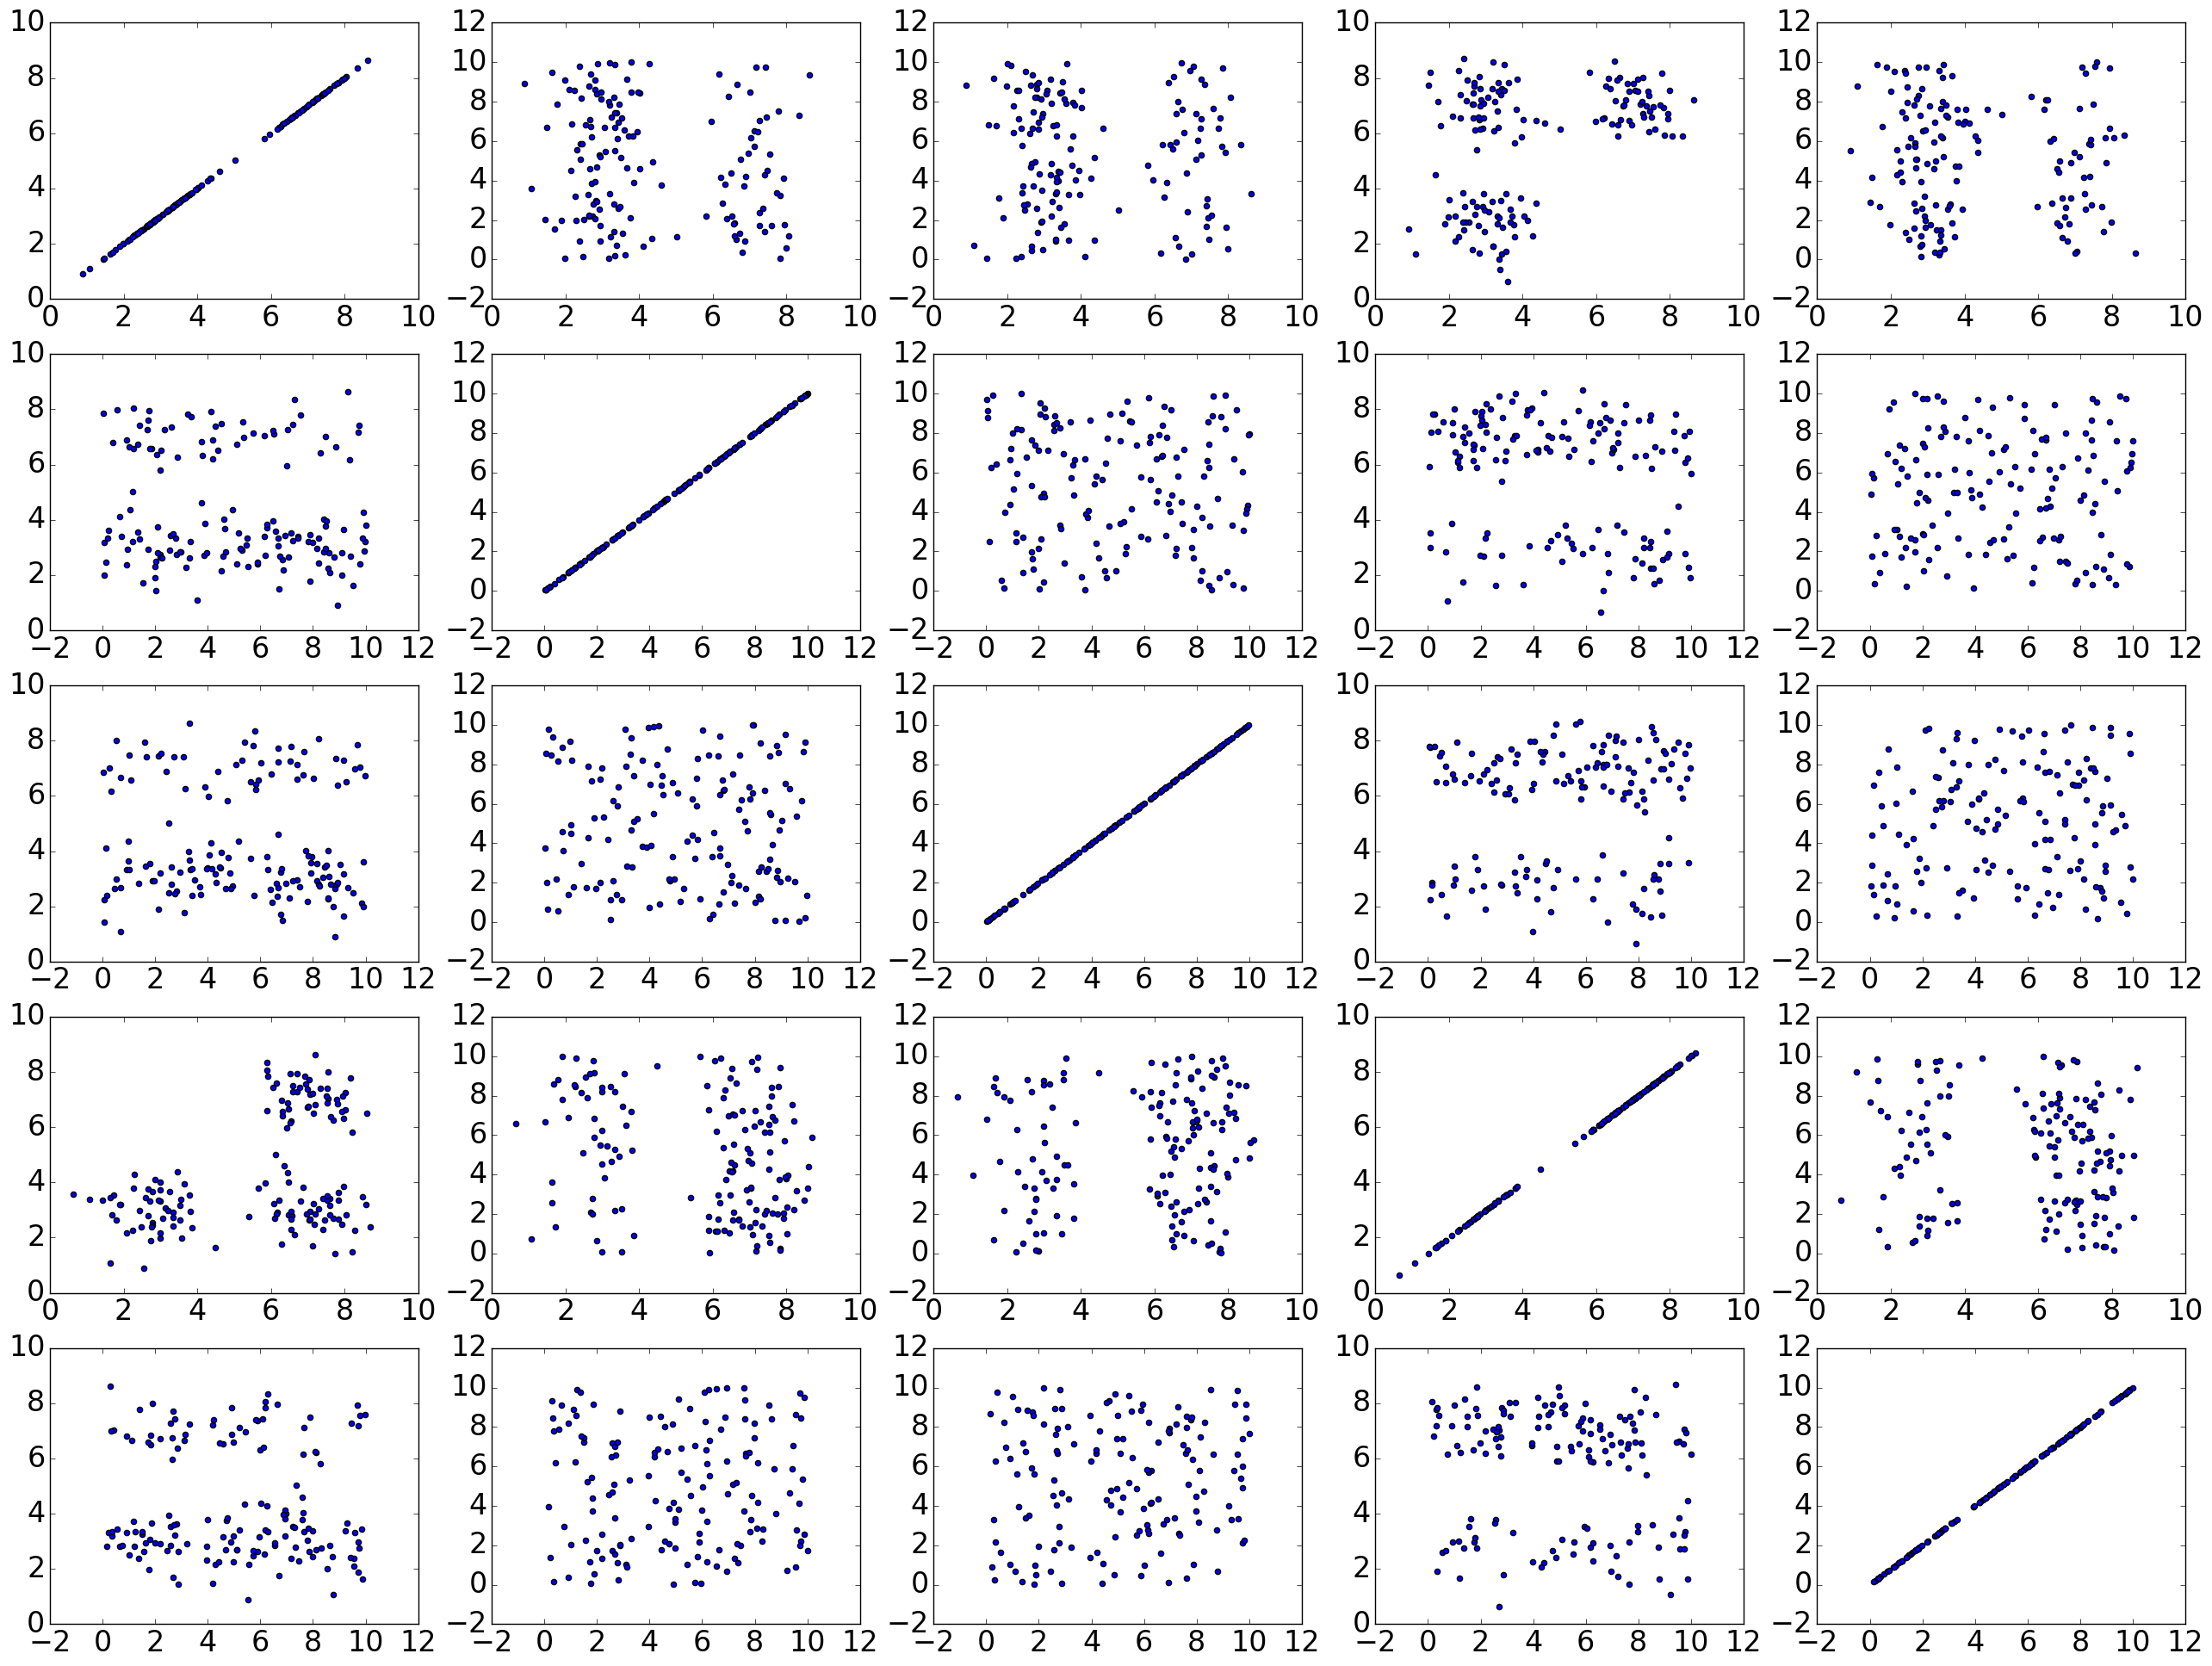
\includegraphics[width=7cm]{attributePlotJosh} }}%
    \qquad
    \subfloat[Dameli]{{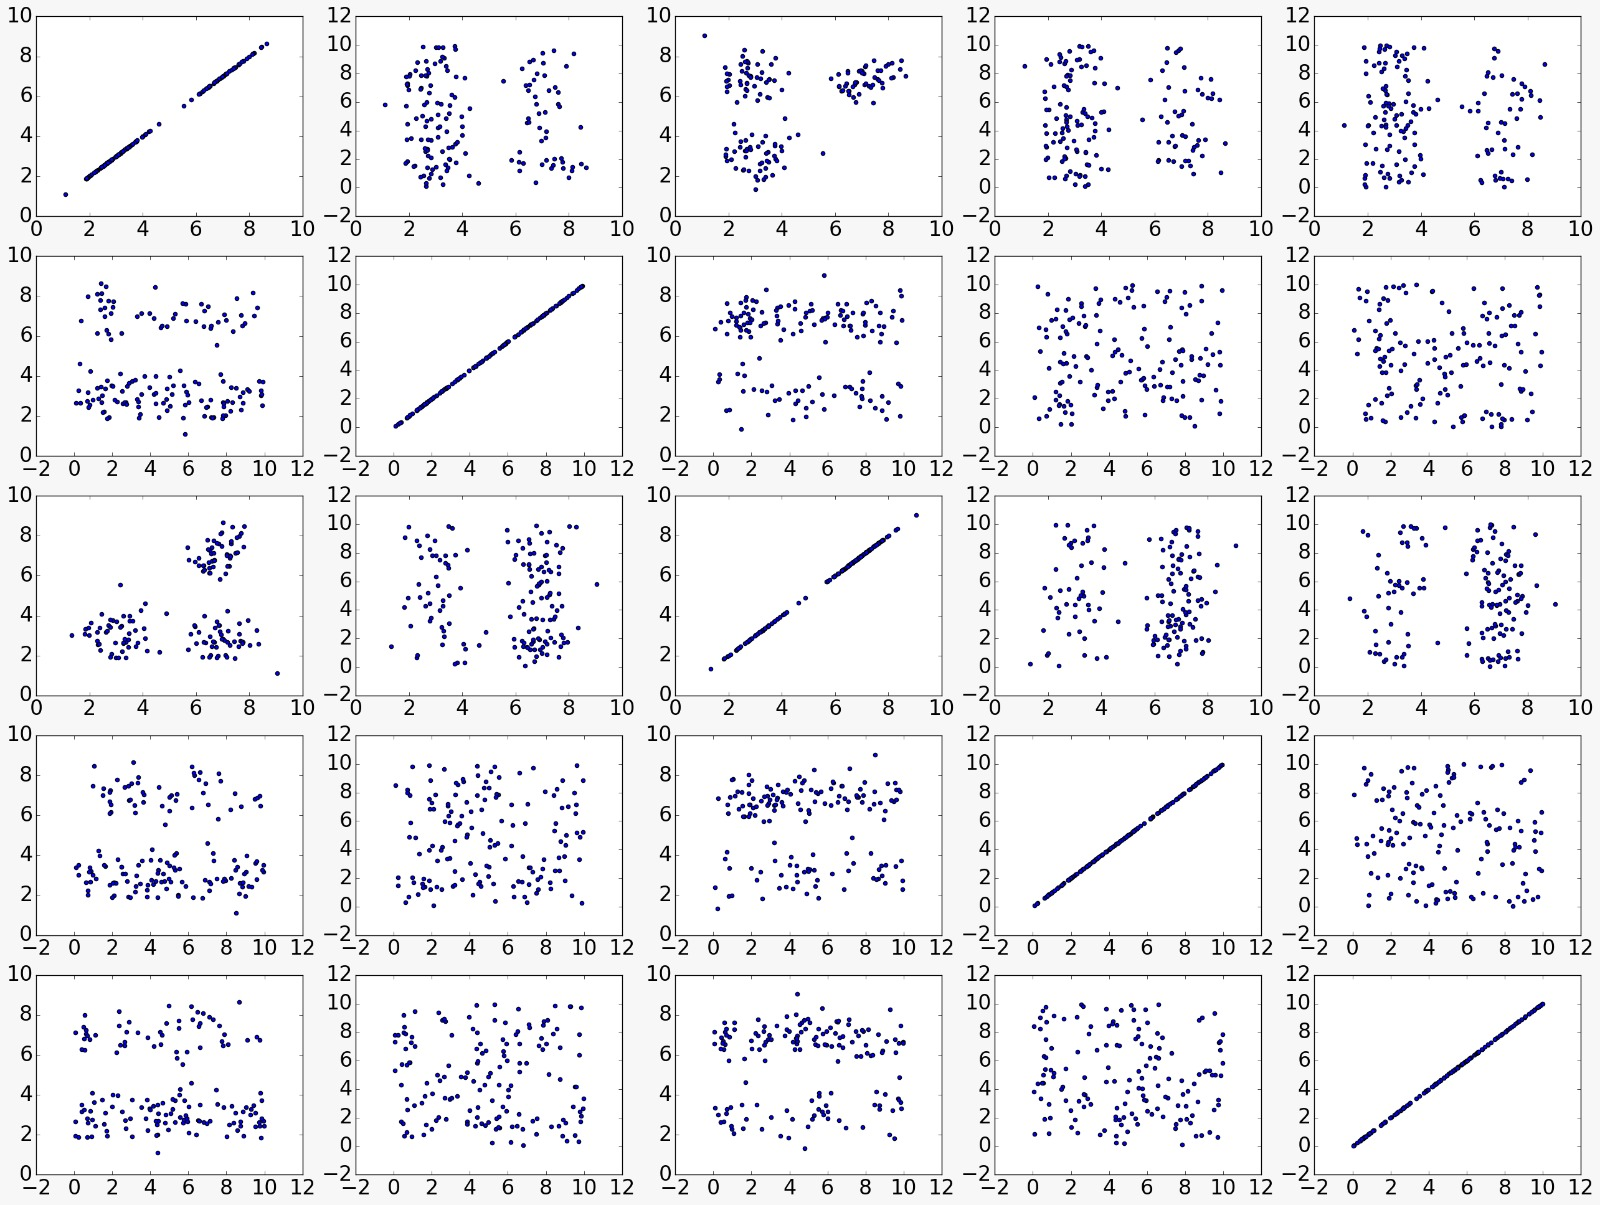
\includegraphics[width=7cm]{attributePlotDameli} }}%
    \caption{Attribute Plots}%
\end{figure}


Inspecting the graphs it is clear that in Figure 1, the attributes that separate the classes into clusters the most for the first set are the first and fourth attribute values whereas the first and fourth attribute values for the second set separate the data into clusters the most. This means that these attributes make up the features of their data sets.


\section*{\vspace{-0.35cm}Identifying the Classes}
Now we have identified that there are three classes displayed by the three clusters we then applied K-means to the data set to obtain the 3 clusters. By using K-means we were able to identify which data points belongs to which clustering. With this information we were able to visualise the different groupings using colour as shown by Figure 2.

\captionsetup[subfigure]{labelformat=empty}
\begin{figure}[h!]
    \centering
    \subfloat[Josh]{{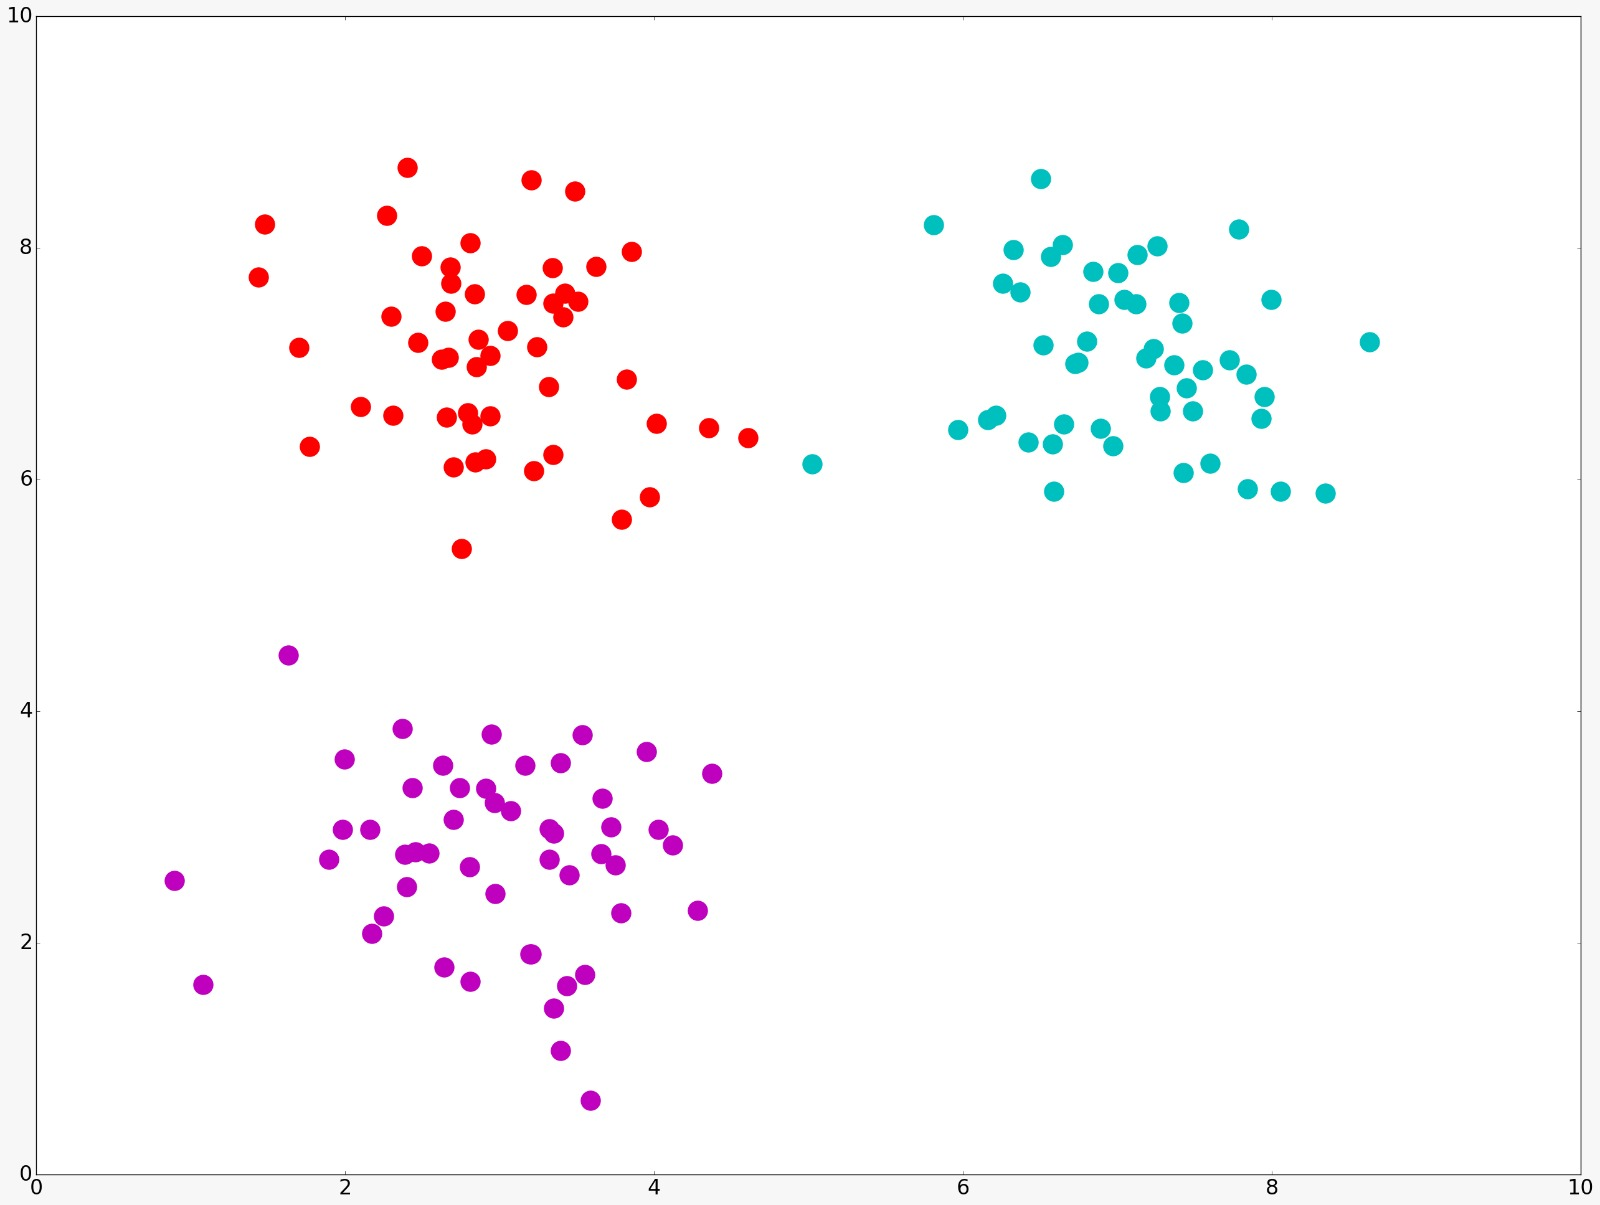
\includegraphics[width=6cm]{clustersJosh} }}%
\end{figure}

The result of visualising K-means and assigning the points to a class is what we expected as it has matched what we thought the clustering should be. K-means is a centroid-based clustering algorithm which partitions features into several sets of data that we refer to, as clusters, by minimising the within-cluster sum of squares. Mathematically, this is denoted as:


\begin{equation*}
  \boldsymbol{\operatorname*{arg\,min}_S} \sum_{i=1}^{k}\sum_{\boldsymbol{x} \epsilon S_i}  \boldsymbol{\parallel x - \mu_{i} \parallel^{2}}
\end{equation*}
According to the number of clusters, n, the algorithm randomly initialises n points that are called centroids. Given that k-means is an iterative algorithm, it iteratively continues doing two steps: assigning a point to a cluster and moving centroids closer to the centre of this cluster. In our case, it will go through each point of the features set and will assign them to one of the cluster groups depending on which cluster is closer to that point. After that, it will recalculate the average of all points within a cluster and will assign the centroid to the current centre of the cluster. The two steps are repeated until the centroid value no longer changes.

\section*{\vspace{-0.35cm}Nearest-centroid Classification}
When classifying new data points into our set one can use the nearest-centroid classification algorithm to fit them into the correct class. We have used our test data set with nearest-centroid to classify the data points into the correct classes. In order to achieve this we obtained the centroids of each class via the K-means algorithm stated before. With

\captionsetup[subfigure]{labelformat=empty}
\begin{figure}[h!]
    \centering
    \subfloat[Josh]{{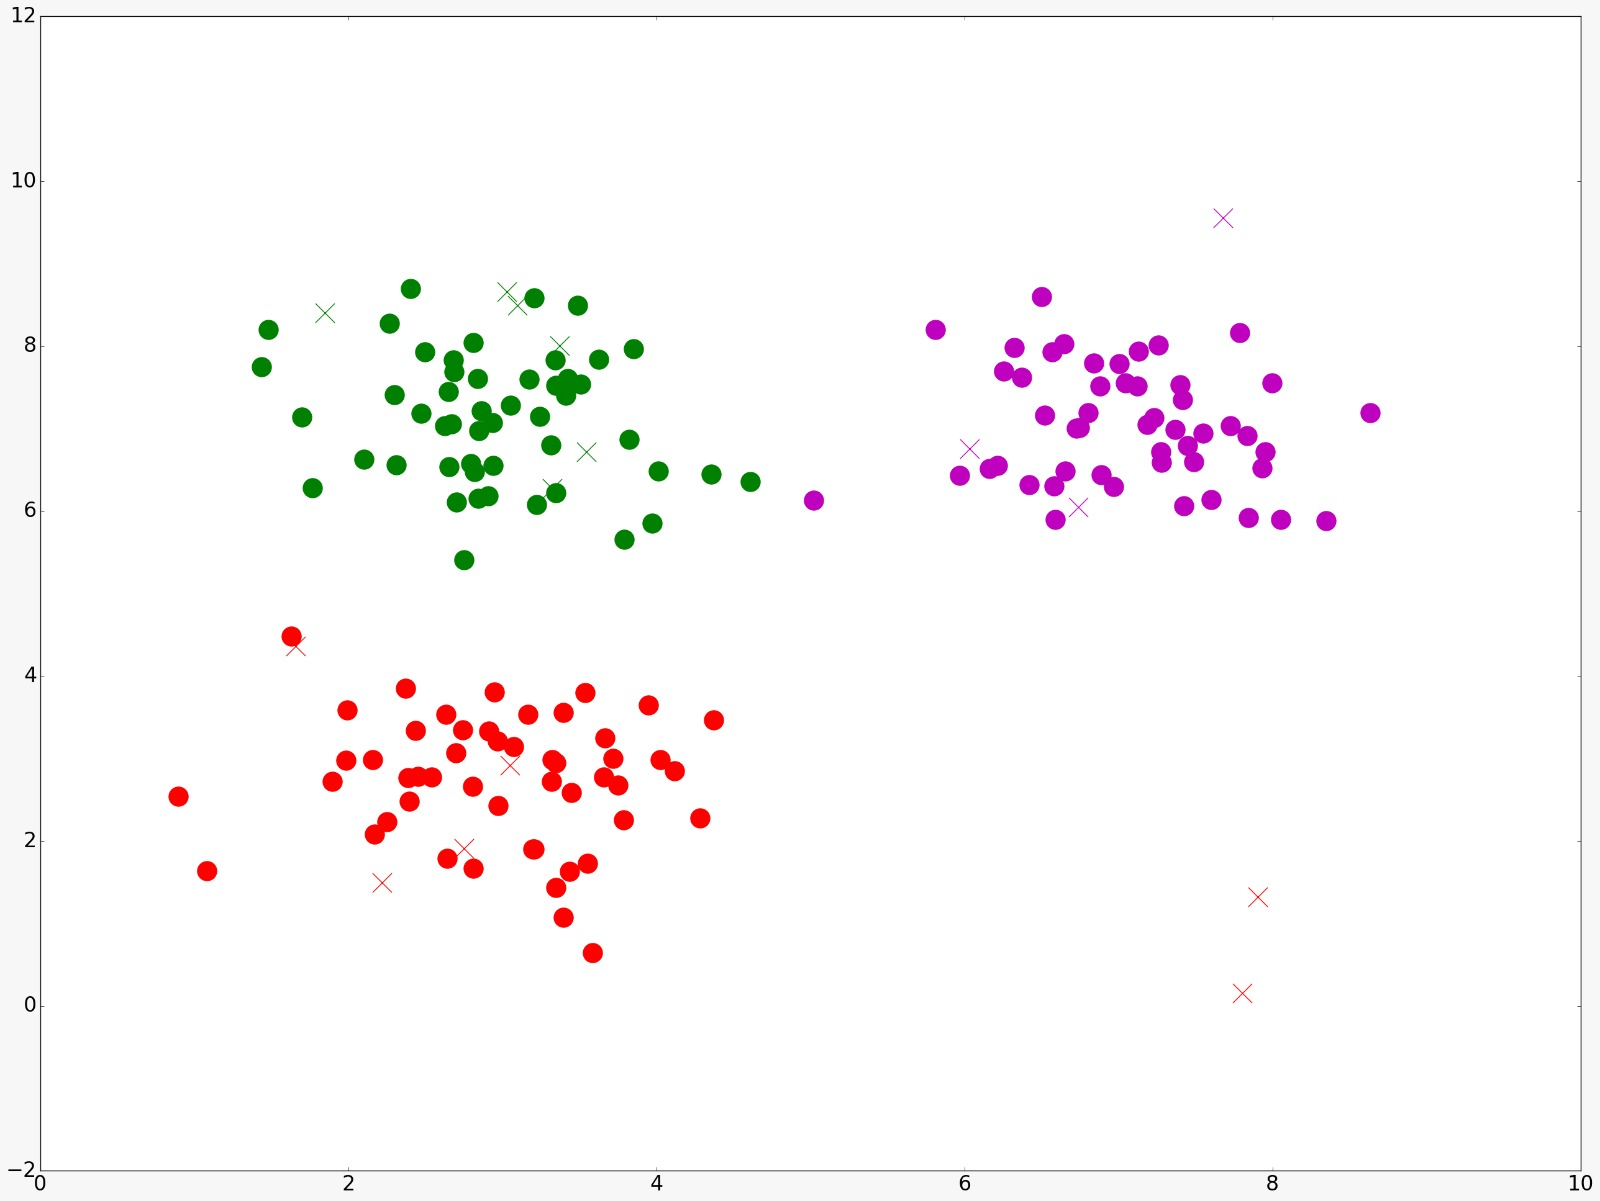
\includegraphics[width=6cm]{testClustersJosh} }}%
    \qquad
    \subfloat[Dameli]{{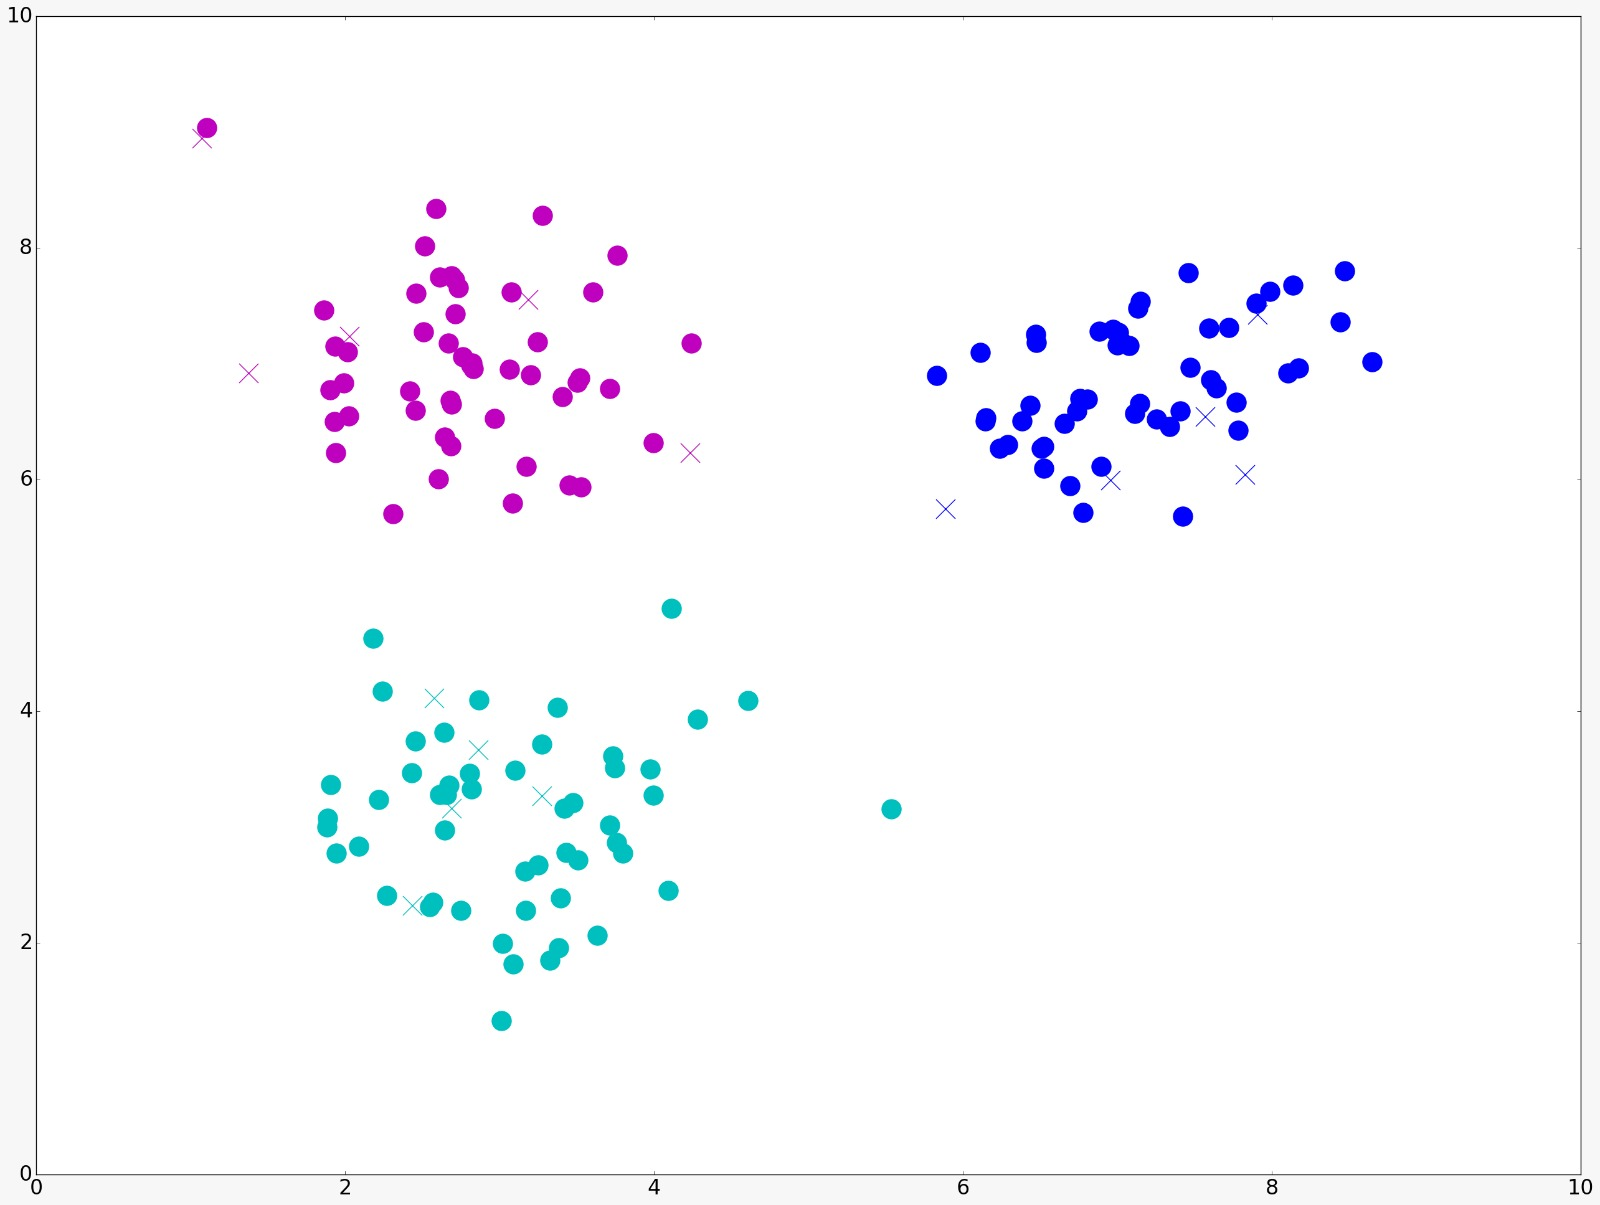
\includegraphics[width=6cm]{testClustersDameli} }}%
    \caption{Nearest-centroid classification}%
\end{figure}

As you can see from the left plot, their are two test data points which are outliers, being a great distance out from any cluster or other points. Even though it is clear that they do not belong in a cluster, and so class, they have still been assigned to the red class. This is because we have specified that there are three clusters that all data points belong to one.


\section*{\vspace{-0.35cm}Maximum-likelihood Classification}

\section*{\vspace{-0.35cm}Discussion of Results}

\begin{thebibliography}{9}
    \bibitem{K-Means}
      K-Means
      \\\texttt{}
\end{thebibliography}

\end{document}
